% % % % % % % % % % % % % % % % % % % % % % % % % % % % % % % % % % % % % % % % % % % %
%                                                                                     %
% Short Sectioned Assignment LaTeX Template Version 1.0 (5/5/12)                      %
% This template has been downloaded from: http://www.LaTeXTemplates.com               %
%                                                                                     %
% Original author:  Frits Wenneker (http://www.howtotex.com)                          %
%                                                                                     %
% Modified by: Fco Javier Sueza Rodríguez (fcosueza@disroot.org)                      %
%                                                                                     %
% Changes:                                                                            %
%	    - Custom Chapters, Sections and Subsections (titlesec package)                %
%           - Document type scrbook (oneside)                                         %
%           - Use babel-lang-spanish package and marvosym                             %
%           - Use hyperref, enumitem, tcolorbox and glossaries packages               %
%           - Use Time New Roman (mathptmx), Helvetic and Courier fonts               %
%                                                                                     %
% License: CC BY-NC-SA 3.0 (http://creativecommons.org/licenses/by-nc-sa/3.0/)        %
%                                                                                     %
% % % % % % % % % % % % % % % % % % % % % % % % % % % % % % % % % % % % % % % % % % % %

%-----------------------------------------------%
%	              Packages                  %
%-----------------------------------------------%

\documentclass[paper=a4, fontsize=11pt, oneside]{scrbook}

% ---- Text Input/Output ----- %

\usepackage[T1]{fontenc}
\usepackage[utf8]{inputenc}
\usepackage{mathptmx}
\usepackage[scaled=.92]{helvet}
\usepackage{courier}
\usepackage[indent=12pt]{parskip}

\usepackage{geometry}
\geometry{verbose,tmargin=3cm,bmargin=3cm,lmargin=2.6cm,rmargin=2.6cm}

% ---- Language ----- %

\usepackage[spanish]{babel}
\usepackage{marvosym}

% ---- Another packages ---- %

\usepackage{amsmath,amsfonts,amsthm}
\usepackage{graphics,graphicx}
\usepackage{titlesec}
\usepackage{fancyhdr}
\usepackage{tcolorbox}
\usepackage{hyperref}
\usepackage{enumitem}
\usepackage[automake]{glossaries}

%--------------------------------------------------------------------%
%                      Customizing Document                          %
%--------------------------------------------------------------------%


% ----------- Custom Chapters, Sections and Subsections -------------- %

\titleformat{\chapter}[display]
			{\bfseries\Huge}
			{Tema \ \thechapter} {0.5ex}
			{\vspace{1ex}\centering}

\titleformat{\section}[hang]
			{\bfseries\Large}
			{\thesection}{0.5em}{}

\titleformat{\subsection}[hang]
			{\bfseries\large}
			{\thesubsection}{0.5em}{}

\titleformat{\subsubsection}[hang]
			{\bfseries\large}
			{\thesubsubsection}{0.5em}{}

\hypersetup{
    colorlinks=true,
    linkcolor=black,
    urlcolor=magenta
}

% ------------------- Custom heaaders and footers ------------------- %

\pagestyle{fancyplain}

\fancyhead[]{}
\fancyfoot[L]{}
\fancyfoot[C]{}
\fancyfoot[R]{\thepage}

\renewcommand{\headrulewidth}{0pt} % Remove header underlines
\renewcommand{\footrulewidth}{0pt} % Remove footer underlines

\setlength{\headheight}{13.6pt} % Customize the height of the header

% --------- Numbering equations, figures and tables ----------------- %

\numberwithin{equation}{section} % Number equations within sections
\numberwithin{figure}{section} % Number figures within sections
\numberwithin{table}{section} % Number tables within sections

% ------------------------ New Commands ----------------------------- %

\newcommand{\horrule}[1]{\rule{\linewidth}{#1}} % Create horizontal rule command


%----------------------------------------------------------------------------------------
%	TÍTULO Y DATOS DEL ALUMNO
%----------------------------------------------------------------------------------------

\title{
\vspace{10ex}
\normalfont \normalsize
\huge \textbf{Tarea 1: Introducción a la Analítica Web}
}
\author{Francisco Javier Sueza Rodríguez}
\date{\normalsize\today}

%----------------------------------------------------------------------------------------
%                                     DOCUMENTO
%----------------------------------------------------------------------------------------
\begin{document}

\maketitle

\thispagestyle{empty}

\vspace{65ex}

\begin{center}
    \begin{tabular}{l l}
        \textbf{Centro}: & IES Aguadulce \\
        \textbf{Ciclo Formativo}: & Desarrollo Aplicaciones Web (Distancia)\\
        \textbf{Asignatura}: & Horas de Libre Configuración\\
        \textbf{Tema}: & Tema 1 -  Introducción a la Analítica Web\\
    \end{tabular}
\end{center}

\newpage

\tableofcontents

\vspace{30ex}

\listoffigures

\newpage

\section{Ejercicio 2}
\subsection{Enunciado}
Publica en el foro de la unidad en el hilo " Mi web/blog"  la dirección de tu sitio web o blog, el objetivo es generar tráfico para que analytics lo registre y obtengas valores. Posteriormente ( si puedes espera un poco para obtener los datos con el fin que se genere tráfico)

Publica en el foro de la unidad en el hilo " Mi web/blog"  la dirección de tu sitio web o blog, el objetivo es generar tráfico para que analytics lo registre y obtengas valores. Posteriormente ( si puedes espera un poco para obtener los datos con el fin que se genere tráfico)

- Usuarios en los últimos 30 min, usuarios por primer medio, Usuarios por audiencia .....

\subsection{Solución}
En esta tarea hemos aprendido a usar Google Analitics. En mi caso, se ha asociado el servicio con la web \href{https://sites.google.com/view/sitewise/inicio}{SiteWise}. Esta web la he creado con Google Sites para la asignatura Empresa e Iniciativa Emprendedora, siendo la web de mi empresa ficticia SiteWise.

Siguiente el proceso descrito en el videotutorial del ejercicio 1, he dado de alta una cuenta de GA y la he enlazado con con la página web. Posteriormente he posteado la web en el foro para que se generará un poco de tráfico.

Tras esperar varios días, se ha generado muy poco tráfico. Como podemos en la siguiente captura del \textbf{informe panorámico}, solo ha habido 2 usuarios. Aunque por lo menos estos nos ha servido para saber que se ha enlazado correctamente la web con GA.

\begin{figure}[H]
    \centering
    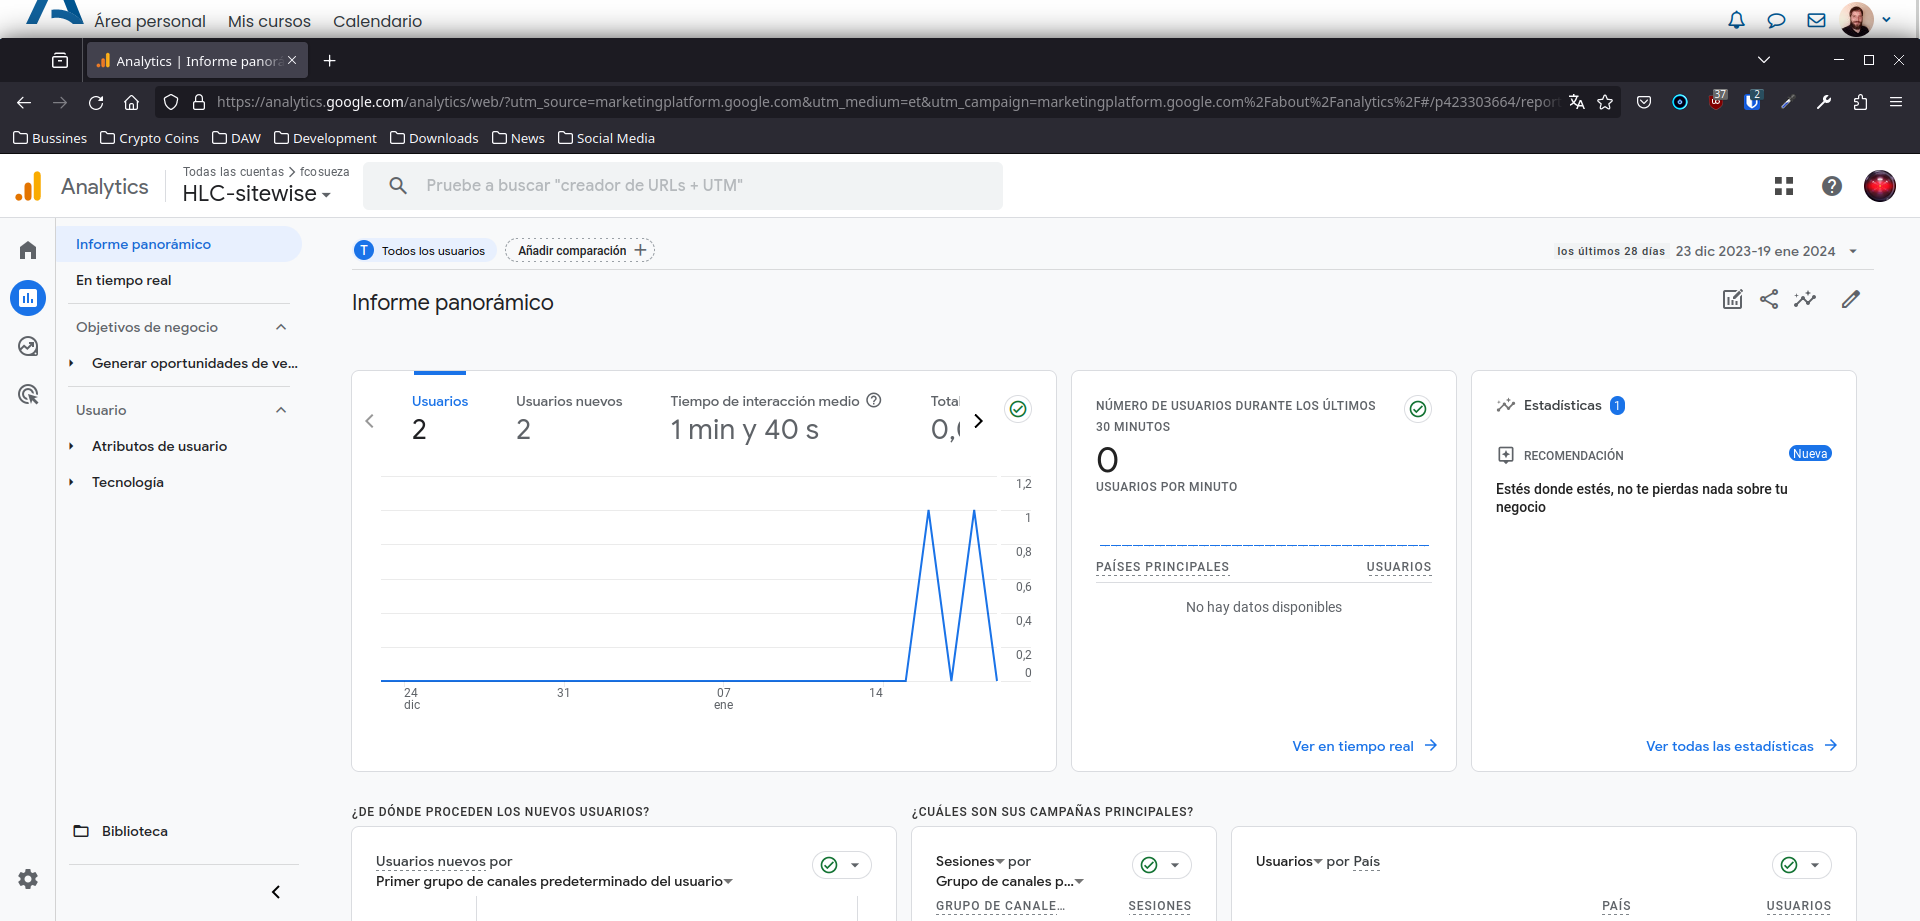
\includegraphics[scale=0.30]{informe-principal.png}
    \caption{Informe panorámico GA}
\end{figure}

Por desgracia en el \textbf{informe de tiempo real} no aparecen datos, ya que no ha habido tráfico en los últimos 30 minutos. A pesar de ello vamos a pasar a explicar cada uno de los datos que se muestran en la secciones de este informe.

En la siguiente figura, podemos ver una captura de pantalla del informe en tiempo real generado por GA, para mi web.

\begin{figure}[H]
    \centering
    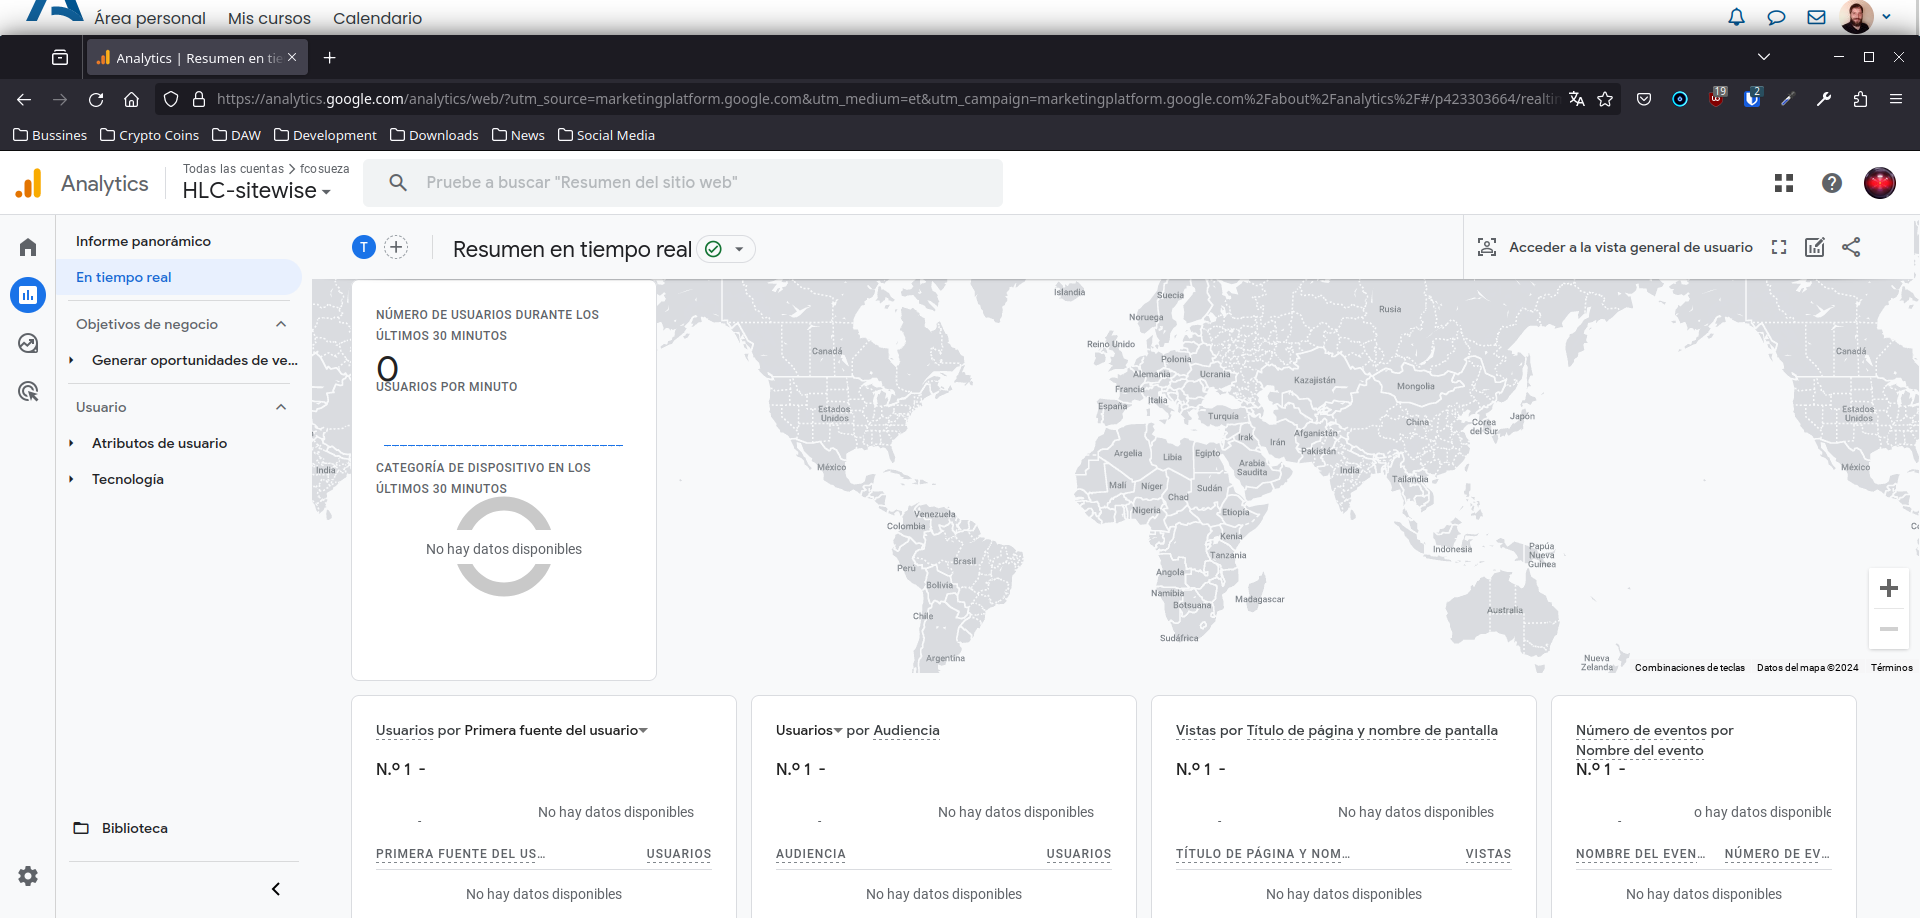
\includegraphics[scale=0.30]{informe-tiempo-real.png}
    \caption{Informe en Tiempo Real GA}
\end{figure}

Como podemos ver en la captura, tenemos diferentes elementos que describimos a continuación:

\begin{itemize}
    \item \textbf{Mapa del Mundo}: este elemento, que ocupa casi la mayor parte de la página, nos muestra los usuario que han usado nuestra página web situados en el mapa del mundo, representados como puntos. Nos sirve para ver de forma rápida y clara como están distribuidos nuestros usuarios a nivel mundial.

    \item \textbf{Usuarios Últimos 30 minutos}: a la izquierda del mapa se nos muestra los usuario que han accedido a nuestra página en los últimos 30 minutos, justo debajo, se nos muestran los dispositivos con los que han accedido estos usuarios a nuestra página.

    \item \textbf{Informes de Usuario}: debajo del mapa y los usuarios de los últimos 30 minutos nos aparecen 6 informes con diferentes información sobre los usuarios. Estos informes son:

    \begin{itemize}
        \item \textbf{Usuarios por Primera fuente/medio/plataforma/campaña del Usuario}: en este informe se nos muestra desde donde vienen nuestros usuario y que medios o plataforma han usado. Por ejemplo, si han sido redirigidos a nuestra página desde una web social, una campaña que hayamos creado, etc... Podemos elegir si se nos muestra la información por fuente, medio, plataforma o campaña de forma individual.

        \item \textbf{Usuarios Por Audiencia}: en este informe se nos muestran grupos de usuario que determinados atributos que podemos crear nosotros. Por ejemplo, usuarios que han visitado la página más de 2 veces, que han comprado X productos, que han realizado más de 3 sesiones en la última semana, etc. Nosotros podemos definir los atributos por los que queremos que se agrupen a los usuarios.

        \item \textbf{Vistas por Titulo de Página y Nombre de Pantalla}: en este informe se muestra el número de páginas que han visitado los usuarios, empleando el título de la página o el nombre de pantalla del desarrollador para contabilizar este dato.

        \item \textbf{Número de Eventos por Nombre de Eventos}: en este informe se nos muestra el número de eventos que han activado los usuarios. Son eventos que podemos definir nosotros mismos y que pueden ser acciones como pulsar un determinado enlace o cargar X veces una página.

        \item \textbf{Conversiones por Nombre de Evento}: en este informe se nos muestran las conversiones por cada evento. Una conversión es un evento que resulta beneficioso para la empresa o página web. Por ejemplo, la compra de un producto o la visualización de un anuncio.

        \item \textbf{Usuarios por Propiedad de Usuario}: por último, este informe nos muestra todos los usuarios agrupados por ciertas propiedades, que podemos especificar, como por ejemplo el idioma preferido, ubicaciones geográficas, rango de edad, etc...
    \end{itemize}
\end{itemize}

Como vemos, \textbf{Google Analitics} nos permite tener una visión muy detallada de los usuarios que visitan nuestra página web y las acciones que llevan a cabo, siendo una herramienta de vital importancia para saber redirigir nuestra web o empresa dependiendo de como nuestros usuarios usan la página.




% Bibliography

%\newpage
%\bibliography{citas}
%\bibliographystyle{unsrt}

\end{document}